\label{fs-acker-preliminaries}

\subsection{Overview}

A substream management system should inform all processes that a substream ends, so the amount of extra traffic cannot be lower than $O(||\Pi||)$. To achieve this lower bound, one can apply an additional agent (process) that receives information about substreams from processes and send them back bound notifications. 

In this case, the fact that substream ends is propagated through this agent without broadcasting between processes, so the amount of extra traffic can be linear by the number of processes. Such propagation method is suitable for cyclic dataflows because there is no need to forward service traffic through the cycles. Therefore, we design a {\em tracking agent} that:

\begin{enumerate}
    \item Receives signals that a substream terminated from data producers.
    \item Watches for in-flight elements and if they belong to some substream.
    \item Notifies dataflow processes when the substream ends {\em for them}, i.e., when they do not receive any elements which satisfy some predicate.
\end{enumerate}

% \tracker\ framework is designed to fit small substreams and cyclic dataflows. It bases on another idea of the propagation the fact that the substream ends. Instead of injecting special elements directly into the dataflow, 

The general scheme of the \tracker\ mechanism is shown in Figure~\ref{tracker_scheme}. Special (possibly distributed) tracking agent receives signals from data sources, fetches information about in-flight elements, and then decides to send notifications about substream end. Before diving into implementation details, we should answer the following questions regarding \tracker\ framework, as explained in the next subsection.

{\bf Q1 How to organize monitoring of in-flight elements?} To detect that a substream ends, the tracking agent should receive the corresponding signal from data producers and ensure no in-flight elements belong to the substream. 

{\bf Q2 How to ensure bound guarantees?} While there are no longer special elements in the stream that denotes the substream end, we need to design other events that indicate the soft and firm substream bound. 

{\bf Q3 How to provide the consistent notifications order?} Unlike punctuations, \tracker\ notifications are completely async with dataflow elements because they go through another network channel. Hence, dataflow items and notifications are not ordered, making it hard to ensure that notifications order is consistent.

{\bf Q4 What are the functional and performance properties of \tracker?} \tracker\ framework is designed to eliminate the limitations of punctuations framework. We should demonstrate that it is suitable for cyclic dataflows as well as can provide lower network overhead.

\begin{figure}[htbp]
  \centering
  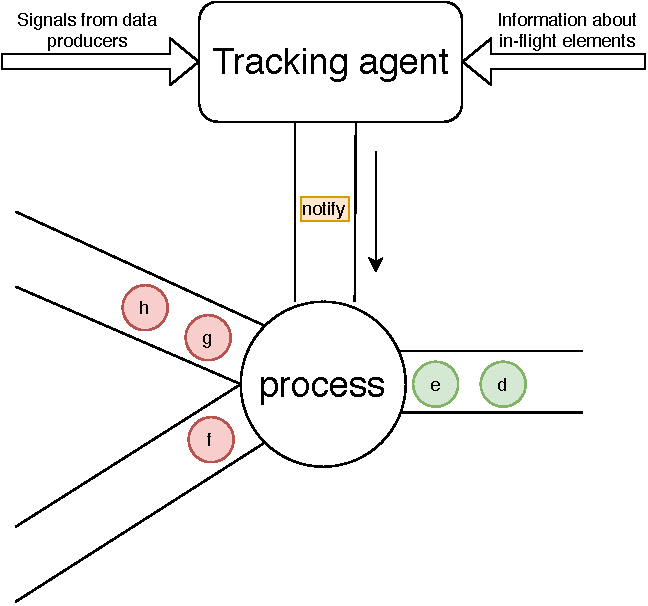
\includegraphics[width=0.35\textwidth]{pics/tracker-scheme.pdf}
  \caption{\tracker\ framework: an example}
  \label{tracker_scheme}
\end{figure}

\subsection{Discussion}

\subsubsection{Answering Q1: How to organize monitoring of in-flight elements?}
Assume that each process sends to tracking agent the following reports about each sending or receiving event $e = <action,m>$:
\begin{enumerate}
    \item $action$: send or receive.
    \item $pred(m)$: the result of applying a substream predicate.
    \item process identifier.
\end{enumerate}

Further in this paper, we will denote them as {\em SND report} and {\em RCV report}. Note that the result of applying predicates can be a vector if we are tracking multiple substreams. Process identifier is an optional field that can be used to send notifications independently for various processes or parts of the physical graph. We will discuss it in detail in the next section.

The tracking agent can monitor the existing substreams: if there are no reports for the specific predicate, the dataflow does not contain elements from the corresponding substream. Using this information along with signals from data producers, the tracking agent can detect when there is a soft guarantee that a substream ends.

A na\"ve implementation of the reports requires an extra network message for each input or output element of a process. However, as we show in the next section, reports can be aggregated and compressed within the process and sent to the tracking agent once per a fixed time period.

\subsubsection{Answering Q2: How to ensure bound guarantees?}

As we mentioned above, tracking agent has enough information to detect the soft substream bound, so it can spawn an {\em end-of-substream event} (EOS), $e^{n} = <send,pred(m)>$. Therefore, function $S(E_{proc})$ for the \tracker\ framework is the following:

\begin{align*}
& S_{tracker}(E_{proc}) = \exists e^{n} \in E_{proc} : e^{n} = \langle recv,pred(m)\rangle_{tracker,p}
\end{align*}

To make this function satisfy the firm notifications guarantee, one needs to block an input channel if the element that does not belong to the substream arrives. After the EOS from the tracking agent arrives, the channel is unblocked. This technique is quite similar to the punctuations alignment, mentioned in the previous section. The processing order function $R_{tracker}(e)$ for this case should satisfy the following condition:

\begin{align*}
& \exists q \in I_p, e = \langle recv,m \rangle_{q,p}: \neg pred(m) \Longrightarrow \\ 
& R_{tracker}(e) > R_{tracker}(e^{n}= \langle recv,pred(m) \rangle_{tracker,p})
\end{align*}

The correctness of the notification guarantees for \tracker\ depends on the implementation of the tracking agent detailed in the next section. The formal proofs that functions $S_{tracker}(E_{proc})$, $R_{tracker}(e)$ along with the \tracker\ implementation satisfy the soft bound and firm bound guarantees are in the appendix~\ref{appendix:tracker-proof}.

\subsubsection{Answering Q3: How to provide the consistent notifications order?}
To provide a consistent order of notifications, one can define a coincident order between notifications and dataflow items. While in punctuations, such order is provided by design, because punctuations and ordinary data items go through the same FIFO network channels, in \tracker\, this order should be artificially defined.

Assume that SPE assigns to input data elements special totally ordered labels $t(m)$, i.e. $\forall q\in \Pi,a\in A, e=\langle send,m\rangle_{aq}, \exists t(m)$. All data elements which are generated from the input item inherit the label: 

$$\forall q\in \Pi, e=\langle proc,m,M_i\rangle_q, \forall x \in M_i : t(x) = t(m)$$.

In this case, if the order on $t(x)$ coincides with the order of input elements, then \tracker\ can produce the EOS events according to this order as well. In other words, \tracker\ can reorder the EOS events such that they will be consistent with the substreams order. An example of this concept is shown in Figure~\ref{tracker_ordering}. The substream containing element with $t(m)=1$ ends before the substream containing element with $t(m)=2$. As we can see, the order of EOS elements from \tracker\ coincides with $t(m)$.

\begin{figure}[htbp]
  \centering
  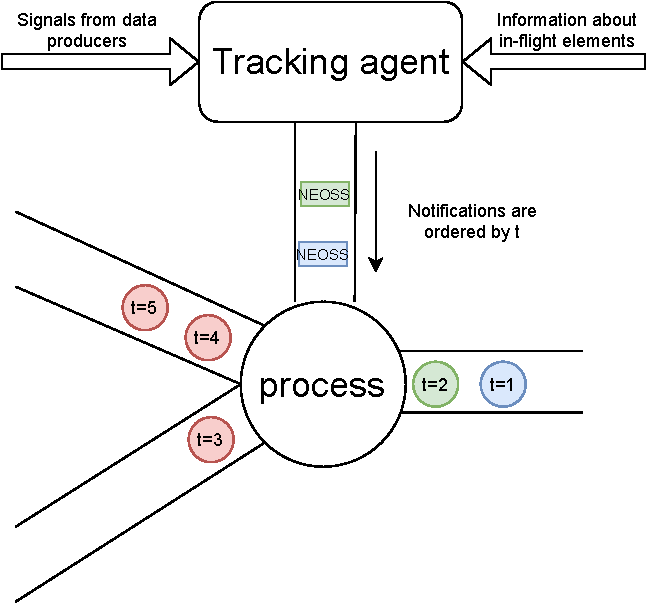
\includegraphics[width=0.35\textwidth]{pics/tracker-ordering.pdf}
  \caption{\tracker\ framework: notifications order}
  \label{tracker_ordering}
\end{figure}

A vital question here is how to implement the assignment of ordered labels $t(m)$. One way is to use the {\em time oracle} service~\cite{10.14778/3055330.3055335} which can provide totally ordered labels. A simple alternative implementation is detailed in the next section. 

\subsubsection{Answering Q4: What are the functional and performance properties of \tracker?}

\tracker\ does not require regular broadcasting of the elements to all computational nodes because all service traffic goes through a single agent. This change of the method of the propagation the fact that the substream ends allows \tracker\ to have the following features by design:

\begin{enumerate}
    \item {\bf Cyclic dataflows support.} Because the tracking agent is monitoring for the properties of in-flight elements without direct injection of service items into a dataflow, \tracker\ does not face the problem of throwing them through a cycle.
    \item {\bf Low network overhead.} As we demonstrate further, processes can send reports once per a fixed time period, so there is a constant time of such reports per a finite substream. The reports require $O(||\Pi||)$ extra messages, while the EOS events $O(K||\Pi||)$. The total amount is $O(K||\Pi|| + ||\Pi||) = O(K||\Pi||)$ that is optimal for the substream management problem. 
\end{enumerate}

At the same time, \tracker\ can provide both soft and firm bound guarantees along with the consistent order of notifications. A limitation of the \tracker\ framework is a potentially more complex implementation than punctuations. The details of the straightforward implementation of the \tracker\ framework are discussed in the next section.
